\documentclass[conference]{IEEEtran}
\IEEEoverridecommandlockouts
% The preceding line is only needed to identify funding in the first footnote. If that is unneeded, please comment it out.
\usepackage{cite}
\usepackage{amsmath,amssymb,amsfonts}
%\usepackage{algorithmic}
\usepackage{textcomp}
\usepackage{xcolor}
\usepackage{balance}
\usepackage{booktabs} % For formal tables
\usepackage{float}
\usepackage{graphicx,url}
\usepackage{soulutf8,color}
\usepackage{lipsum}
\usepackage{stfloats}
\usepackage{verbatim}
\usepackage[utf8]{inputenc}  
% UTF-8 encoding is recommended by ShareLaTex
\usepackage[inline]{enumitem}
\usepackage{multirow}
\usepackage{array}
\usepackage{tikz}
\usepackage{hyperref}
%\usepackage[brazil]{babel}
\newcommand*\numcircledtikz[1]{\tikz[baseline=(char.base)]{
            \node[shape=circle,fill=green,draw,inner sep=1.2pt] (char) {#1};}}
\def\BibTeX{{\rm B\kern-.05em{\sc i\kern-.025em b}\kern-.08em
    T\kern-.1667em\lower.7ex\hbox{E}\kern-.125emX}}

\renewcommand{\abstractname}{Resumo}
\renewcommand{\refname}{REFERÊNCIAS}
\renewcommand{\tablename}{TABELA}

\begin{document}


%\title{Avaliação de Desempenho, Custo e Tempo de Inicialização de uma Função Serverless na AWS ao Comparar a Implantação Através de Arquivo Compactado e Via Imagem de Contêiner}

\title{Análise comparativa de modelos de implantação de funções \textit{serverless} no serviço AWS Lambda}

\author{\IEEEauthorblockN{%1\textsuperscript{st}
Gabriel Duessmann}
\IEEEauthorblockA{\textit{Programa de Pós-Graduação em Computação Aplicada} \\
\textit{Universidade do Estado de Santa Catarina}\\
Joinville, Brasil \\
gabriel.duessmann@edu.udesc.com}
\and
\IEEEauthorblockN{%2\textsuperscript{nd}
Adriano Fiorese}
\IEEEauthorblockA{\textit{Departmento de Ciência da Computação } \\
\textit{Universidade do Estado de Santa Catarina}\\
Joinville, Brasil \\
adriano.fiorese@udesc.br}
}

\maketitle

\begin{abstract}

Com o avanço da computação em nuvem as tradicionais formas de desenvolvimento de serviços de software vem sendo atualizadas bem como novas vem sendo desenvolvidas. É o caso de serviços "sem servidor" ou \textit{serverless}, que vem ganhando atenção. Nesse caso, provedores de serviços em nuvem oferecem serviços de hospedagem e execução \textit{serverless}. Em particular, a empresa Amazon disponibiliza o AWS Lambda para a criação de funções \textit{serverless} pelos seus clientes. Existem ao menos duas formas de implantação de funções \textit{serverless}. Uma forma encapsula o código fonte e demais arquivos necessários em um arquivo compactado no formato ZIP, e outra onde a própria função executável e demais dependências estão em uma imagem de contêiner. Dependendo da abordagem escolhida, o desempenho, o custo e o tempo de inicialização podem variar. Levando em consideração essas métricas, este trabalho visa comparar essas duas abordagens de implantação de funções \textit{serverless} e tem como objetivo descobrir se uma das abordagens apresenta ser mais adequada do que outra. Experimentos conduzidos visando tal comparação demonstram que a criação de funções utilizando arquivo compactado ZIP apresentam vantagens, principalmente no tempo de inicialização da função quando 
em modo de partida fria. 
\end{abstract}

\begin{IEEEkeywords}
Função Serverless, AWS Lambda, Contêiner, Avaliação, Desempenho, Custo, Tempo Inicialização
\end{IEEEkeywords}

%===================================================================

\section{Introdução}
\label{sec:Intro}

\textit{Serverless} é um modelo de computação em nuvem na qual os provedores ofertam serviços para provisionar  dinamicamente servidores configurados para que seus clientes executem suas aplicações, assumindo a responsabilidade de provisionamento, escalabilidade e segurança das aplicações \cite{Nupponen_2020_serverless_what_it_is}.
Isso se torna prático para que os desenvolvedores e as companhias implementem suas aplicações sem precisar configurar a infraestutura necessária para sua execução, mesmo que em nuvem. 
Cada aplicação implantada nesse modelo, é chamada de função \textit{serverless}, que executa o código independentemente da infraestrutura.

Ao comparar o modelo \textit{serverless} com aplicações monolíticas, as aplicações \textit{serverless} são menores, não precisam de configurações de servidor e são nativamente escaláveis com bas com base na utilização dos recursos alocados. Já aplicações monolíticas compõem todo o código de uma aplicação, e por isso tendem a ter uma grande base de código, incluindo configurações de servidores e banco de dados. Portanto, a escalabilidade, além de não ser padrão, pode ser um desafio devido ao maior tamanho da aplicação e necessidade de recursos alocados, visto que esse tipo de aplicação geralmente necessita adicionar mais recursos ao(s) sevidor(es) independente se o gargalo está em apenas uma pequena parte da aplicação.

Apesar das vantagens de se utilizar o paragidma \textit{servless}, como a abstração da infraestutura e o atendimento da demanda elástica da aplicação, a implantação do mesmo demanda cuidados, pois configurações do ambiente são feitas pelo provedor e os desenvolvedores não tem acesso para alterá-las. Tais cuidados estão relacionados a forma em que a aplicação é instanciada e desativada de acordo com o seu uso e ociosidade. 

A medida que a aplicação fica ociosa por um período de tempo (normalmente minutos), cujo tempo é determinado pelo provedor, seu recurso computacional é desalocado, e a mesma fica inoperante. Quando a função se encontra nesse estado, e o cliente realiza uma nova requisição, o serviço é instanciado novamente com os devidos recursos alocados; porém é perceptível um tempo de resposta maior na primeira requisição, devido ao tempo de alocação de recursos.   

No provedor de nuvem AWS, particularmente, há duas maneiras de se implantar uma nova função, que são: a maneira mais tradicional via arquivo compactado (ZIP), ou através de uma imagem de contêiner, opção introduzida pela empresa em 2020 \cite{aws_2020_supports_container_image}.

Na implantação via arquivo compactado, o desenvolvedor precisa compactar a pasta do projeto em formato ZIP, incluindo o código fonte e os arquivos executáveis da aplicação, e deve realizar o \textit{upload} direto para o serviço \textit{serverless}. Com o uso de imagem de contêiner, é necessário conter um arquivo Dockerfile no projeto com as dependências e configurações para realizar o \textit{build} da imagem e executar o projeto. A partir da imagem gerada no ambiente local do desenvolvedor, esta deve ser publicada no repositório de imagens do provedor. Finalmente, para criar a função \textit{serverless}, deve ser selecionada a respectiva imagem disponível no repositório. 

Independente do modelo de implantação escolhido, o desenvolvedor precisa implementar no código da aplicação uma interface fornecida pela AWS. Essa interface tem como objetivo definir o método de entrada para qual será enchaminhado as requisições recebidas, assim como os parâmetros de entrada e saída. Dessa forma, a função \textit{serverless} sabe qual método do código invocar ao receber requisições.

Sendo assim, este trabalho aborda as duas possibilidades de implantar funções \textit{serverless} na AWS e propõe uma comparação de desempenho, custo e tempo de inicialização entre as abordagens. Por fim, busca-se concluir se há um modelo de implantação mais vantajoso do que outro.

Para chegar nos resultados de comparação, testes foram executados nas funções \textit{serverless} via chamadas de API. As métricas analisadas foram de consumo máximo de memória, o custo para implantar as funções e o tempo de inicialização da aplicação. Durante a execução de testes, não houve cobrança nos serviços utilizados, por ter sido utilizado o modelo \textit{Free Tier}. Portanto, a comparação de custo foi baseada nos valores e cáculos informados pela Amazon.

Esse artigo é estruturado da seguinte maneira: A Seção \ref{sec:RefTeo} apresenta o referencial teórico para esclarecer termos relacionados a nuvem e ao provedor AWS, e apresentar características utilizadas na avaliação. A Seção \ref{sec:TrabRel} lista trabalhos relacionados pertinentes ao tema, bem como suas características e como se diferem desse artigo. Na Seção \ref{sec:experiments}, é apresentado a proposta da avaliação, bem como os experimentos realizados e as métricas coletadas. Por fim, a Seção \ref{sec:Conclusion} conclui o artigo.

\section{Referencial Téorico} 
\label{sec:RefTeo}

Com o avanço da computação em nuvem, cada vez mais serviços estão sendo migrados ou implementados nesse modelo. Os provedores de nuvem, por sua vez, estão dedicados a criarem e disponibilizarem recursos que melhoram a qualidade e praticidade de seus serviços a fim de atender um maior conjunto de clientes. Um desses serviços é chamado \textit{serverless}, que executa uma aplicação sem que o cliente necessite configurar o servidor e demais infraestruturas. A implantação de uma aplicação em \textit{serverless} é chamada de função \textit{serverless}. Para que a aplicação seja executada como um função, o desenvolvedor precisa adicionar em seu código as dependências disponibilizadas pelo provedor. Em específico, a implementação necessária para a AWS é abordada na Seção \ref{subsec:aws_services}.
    
\subsection{Computação em Nuvem}
\label{subsec:cloud}

A computação em nuvem é um modelo com vastos recursos de computação compartilhados, como rede, servidores, armazenamento, aplicações e serviços que podem ser provisionados rapidamente e liberados com baixa configuração e complexidade \cite{nist_2011_cloud_computing}.
Os provedores de nuvem são responsáveis por cuidar, controlar e ofertar serviços em nuvem para usuários finais ou entidades. Conforme os clientes utilizam os serviços ofertados, pagam sob demanda de acordo com a utilização dos mesmos ou conforme acordo firmado com o provedor. Com a computação em nuvem, \textit{data centers} e infraestruturas de empresas começaram a ser migrados para nuvem devido a agilidade e praticidade dos serviços ofertados pelos provedores. Como consequência, as aplicações também precisaram ser migradas, o que leva a novas formas de aproveitamento dos recursos computacionais disponíveis, tendo em vista a otimização dos mesmos e do custo, dado o modelo de precificação baseado no pagamento do que é usado sob demanda.

\subsection{Função serverless}
\label{subsec:serverless_funcion}

Funções \textit{serverless} ou modelo Function as a Service (FaaS) providenciam a abstração dos servidores e demais infraestrutura. Os clientes do modelo, ou seja, os desenvolvedores de aplicações, precisam apenas implementar o código da aplicação, isto é, a função. Ao ter o código implementado, é responsabilidade do provedor instanciar o servidor físico ou virtual, configurar o ambiente e disponibilizar uma Application Program Interface (API) para acesso da aplicação por parte do cliente da mesma. 

Uma das principais vantagens desse modelo é que o provedor é responsável pela escalabilidade da aplicação. A escalabilidade nesse caso contempla a instanciação da função para sua utilização pelos clientes da aplicação, de forma a atender a demanda de requisições, bem como o gerenciamento dessas instâncias quando não estão necessariamente atendendo às requisições dos clientes finais. É possível utilizar estratégias de otimização com vistas a reutilização dos recursos para o atendimento da escalabilidade.
Uma das estratégias utilizadas para gerenciar o dimensionamento dos recursos é chamada de \textit{cold start}, ou partida lenta. 
Conforme a função deixa de ser utilizada, os recursos de \textit{hardware} alocados passam a ficar ociosos, e portanto, os provedores desalocam parte desses recursos para obter uma maior economia. Quando a aplicação é novamente invocada, pode necessitar que os recursos sejam reativados e uma nova instância seja criada. Esse processo é chamado de partida lenta ou fria \cite{vahidinia_2020_cold_start}. Após ter os recursos reativados, essa instância permanecerá ativa enquanto é utilizada, e por um período de tempo após a sua utilização, processo que é chamado de partida quente, pois possui a instância e os recursos operantes \cite{Raje_2023_cold_warm_start} para o atendimento de nova requisição, sem que se instancie uma nova instância da função. A função, após ficar alguns minutos ociosa, sem nenhuma execução, tem seus recursos desativados pelo provedor. Esse ciclo continua alternando entre partida fria e partida quente conforme a utilização pelos usuários finais.

Otimizações para diminuir o tempo da partida lenta são estudados para evitar grandes atrasos ao cliente final apesar da dificuldade de alcançar soluções ideais, dado que as configurações acerca do gerenciamento dos recursos e das instanciações são mantidas pelos provedores de nuvem \cite{vahidinia_2020_cold_start, kumari_2022_mitigating_cold_start, vahidinia_2023_mitigating_cold_start, dantas_2022_reducing_cold_start}, e não são disponíveis para experimentações e otimizações por parte dos desenvolvedores da aplicação.

\subsection{Contêineres}
\label{subsec:containers}

Contêineres fornecem às aplicações um ambiente configurado com todas as suas dependências para ser executado. Eles isolam a aplicação de programas e processos externos que executam no sistema operacional hospedeiro. Portanto, pode ser definido como um mecanismo de empacotamento de aplicações \cite{Siddiqui_2019_analysis_container}. 

A utilização de contêineres se tornou amplamente popular pela facilidade de migrar aplicações de um ambiente para outro sem a ocorrência de problemas ao executar em máquinas diferentes. Sem isso, toda vez que as aplicações migravam para um novo ambiente, havia uma grande chance de ocorrerem erros, pois dois ambientes nunca são totalmente idênticos em questão de \textit{software} e \textit{hardware}, e portanto, podem não ter as configurações e dependências necessárias para a execução da aplicação  \cite{Siddiqui_2019_analysis_container}. Sem o uso de contêineres ou alguma técnica de virtualização, ou seja, em \textit{bare metal}, para cada vez que a aplicação executasse em uma máquina diferente, seria necessário antes disso, instalar suas dependências, programas de terceiro, configurar o ambiente, entre outros.

Para que uma aplicação seja portável entre máquinas com contêiner, é preciso de uma imagem da aplicação com tudo o que é necessário para executá-la. Com a imagem criada, o contêiner pode ser replicado para outras máquinas de diferentes \textit{hardwares} e sistemas operacionais (SOs), mantendo o mesmo funcionamento da aplicação. Isso é possível porque os contêineres são uma forma de virtualização leve, que pode incluir seu próprio SO. \cite{scheepers_2014_virtualization_containerization}. Sendo assim, pode-se ter uma imagem de contêiner para cada função \textit{serverless} que se deseja criar e especificar qual imagem utilizar ao criar uma nova função no AWS Lambda. 


\subsection{Serviços AWS}
\label{subsec:aws_services}

Um dos maiores provedores de nuvem da atualidade é a AWS (Amazon Web Service), que oferta centenas de serviços disponíveis na Internet. Dentre os serviços ofertados, este trabalho utiliza três deles: AWS Lambda, API Gateway e AWS ECR.

O serviço de \textit{serverless} da Amazon é chamado de AWS Lambda, e nele, consegue-se criar funções para executar aplicações sem precisar provisionar e gerenciar servidores. 
O serviço Lambda gerencia toda a configuração computacional, que oferece equilíbrio de memória, CPU, rede e outros recursos necessários para executar o código da aplicação (função).
As funções são instanciadas sob demanda conforme requisições feitas por usuários finais, o que faz o serviço alocar parte da máquina virtual para a função. Conforme a função passa a ficar ociosa por alguns minutos, os recursos computacionais alocados são desativados. Isso possibilita que os clientes paguem apenas pelo tempo em que a aplicação está sendo utilizada, com os recursos alocados para a função \textit{serverless} \cite{aws_2023_what_is_lambda}.

Para implantar uma aplicação em função \textit{serverless}, é necessário que o desenvolvedor importe em seu projeto as bibliotecas da AWS Lambda especificas para cada linguagem de programação e implemente a interface do serviço \textit{serverless} disponibilizada pela biblioteca específica. Ao criar a função, na etapa de configuração, é necessário informar o caminho do método que implementa a interface, pois esse método é usado como ponto de entrada para a função invocar a aplicação e passar os parâmetros de entrada.

Particularmente, na AWS, há duas maneiras de implantar uma função \textit{serverless}, que são: via arquivo compactado do código fonte ou com uma imagem de contêiner. Para a abordagem de arquivo compactado, é necessário compilar os arquivos fontes, compactar a pasta do projeto em formato ZIP e fazer o \textit{upload} direto no serviço AWS Lambda. Com o uso de uma imagem de contêiner, é necessário que o desenvolvedor tenha a imagem publicada na AWS ECR (Elastic Container Registry), que é o repositório de imagens de contêineres, e selecionar a respectiva imagem quando da criação da função.

Além das características citadas acerca do servico AWS Lambda, e seus coadjuvantes relacionados ao modelo \textit{serverless}, a arquitetura de \textit{hardware} onde é executada a função também pode ser escolhida junto ao provedor AWS. Assim, ao criar uma nova função, esta pode ser criada sob arquitetura arm64 ou x86\_64. Apesar da arquitetura x86\_64 ser a padrão, a arquitetura arm64 se destaca por possui menor custo de execução e atingir melhores resultados de desempenho
\cite{aws_2023_aws_lambda_architectures}.

AWS ECR é um serviço de repositório para armazenar imagens de contêineres. O desenvolvedor deve criar a imagem em sua máquina local a partir de um arquivo Dockerfile e publicá-la no repositório \cite{aws_2023_aws_ecr}. Ao ter a imagem disponível no repositório, esta pode ser usada em outros serviços do provedor, como por exemplo para criar funções \textit{serverless}.

Amazon API Gateway é um serviço para criar, publicar e gerenciar APIs, podendo ser REST, HTTP ou WebSocket. É usado como um ponto de entrada para os serviços AWS, incluindo o AWS Lambda, e as APIs podem ser criadas para acessarem os serviços criados ou dados armazenados. Esse serviço lida com as tarefas de aceitar e processar as requisições, com capacidade de processar centenas de milhares de requisições concorrentes \cite{aws_2023_what_is_api_gateway}. 

\section{Trabalhos Relacionados}
\label{sec:TrabRel}

Modelos FaaS não são tão recentes, e apesar de trazerem praticidade para implementação de aplicações, há ainda espaço para estudos analisarem pontos de melhoria.

O trabalho \cite{dantas_2022_reducing_cold_start} aborda estratégias para diminuir o \textit{cold start} e compara o impacto no tempo ao instanciar uma função através de arquivo compactado e via imagem de contêiner. Apesar de propor soluções para minimizar o tempo de inicialização, o trabalho citado não aborda custo.

Em \cite{Elsakhawy_2021_performance_analysis_serverless}, são investigados os fatores que afetam o desempenho de funções \textit{serverless} e como também são examinados os resultados em opções de contêineres, diferentes linguagens de programação e alternativas de compilações. Porém, os autores do trabalho citado não levam em consideração o custo para executar a função e tempo de inicialização do \textit{cold start}.

Na publicação \cite{Villamizar_2017_cost_comparison_lambda}, os autores compararam os custos de executar aplicações em monolito, microserviço e função Lambda na AWS. Das três arquiteturas, AWS Lambda obteve o menor custo, reduzindo os custos de infraestrutura em 70\%.

A Tabela \ref{tab:related_papers} compara características de alguns trabalhos relacionados e pontua como esse artigo se difere dos demais. As colunas de arquivo compactado e imagem de contêiner são referentes ao modo de implantação da aplicação. As demais colunas apresentam desempenho, custo e tempo de inicialização como métricas referentes às funções.


\begin{table*}[htb]
    \centering
    \caption{Comparação de trabalhos relacionados}
    \label{tab:related_papers}
    \begin{tabular}{cccccc}
        \hline
         Artigo & Arquivo compactado & Imagem de contêiner & Desempenho & Custo & Tempo de inicialização \\
        \hline
         Dantas\cite{dantas_2022_reducing_cold_start} & Sim & Sim & Não & Sim & Sim \\
        \hline
         Elsakhawy\cite{Elsakhawy_2021_performance_analysis_serverless} & Não  & Sim & Sim & Sim & Não \\
        \hline
         Villamizar\cite{Villamizar_2017_cost_comparison_lambda} & Não & Não & Não & Sim & Não \\
        \hline
         Trabalho atual & Sim & Sim & Sim & Sim & Sim \\
        \hline
    \end{tabular}   
\end{table*}

\section{Experimentos}
\label{sec:experiments}

Este trabalho propõe avaliar dois métodos de implantação de aplicações em serviço \textit{serverless} da Amazon, AWS Lambda.
A linguagem de programação escolhida para o experimento foi Java, devido a sua popularidade no mundo Web e facilidade de implementar as interfaces requeridas para executar a aplicação como função \textit{serverless}.

Devido ao aumento do uso de funções \textit{serverless} nos últimos anos, estudos de otimizações e melhorias vem sendo propostos. Sendo assim, visto que que há dois modelos de implantação de funções \textit{serverless} na AWS, este trabalho busca descobrir se uma das abordagens apresentar ser mais vantajosa. 
Para chegar em tal conclusão, métricas pertinentes ao serviço foram colhetadas e analisadas. As métricas levadas em consideração foram: desempenho com base no consumo de memória, custo e tempo de inicialização em partida lenta. 

Para realizar a comparação das métricas, foram implantados projetos como função \textit{serverless} na AWS Lambda via arquivo ZIP e imagem de contêiner, de forma a obter os dados referentes a cada modelo.

A seguir, é descrito o ambiente e as configurações para simular os testes, e posteriormente são apresentados os dados colhetados de cada métrica.


\subsection{Ambiente}
\label{subsec:environment}

O ambiente de configuração foi realizado exclusivamente na AWS, no qual foram utilizados serviços para uso de funções \textit{severless}, comunicação externa de API via HTTP e coleta de métrica. 

Primeiramente, foram escolhidos projetos para serem a base da função \textit{serverless} do experimento. O primeiro projeto foi o algoritmo de ordenação \textit{bubble-sort}, visto que é um algoritmo simples e pequeno de ser implementado.
Como há uma limitação na AWS Lambda para fazer o \textit{upload} direto de um arquivo compactado de até 10 Mb, o segundo projeto escolhido foi o \hl{projeto X, cujo possui escopo maior e demanda maior processamento computacional}. Para implantação de projetos maiores de 10 Mb, a pasta compactada deve ser enviada para o AWS S3, onde a mesma é armazenada e usada para a criação da função.

Para o primeiro projeto, foi realizado o \textit{build} e gerado as classes executáveis. Após isso o projeto foi compactado em formato ZIP e feito o \textit{upload} direto para AWS Lambda. Para a implantação via imagem de contêiner, um arquivo Dockerfile foi adicionado ao projeto, realizado o \textit{build} da imagem no computador local e enviado a imagem criada para o repositório AWS ERC. Com a imagem disponível do repositório, a mesma foi usada para a implantação da função \textit{serverless}.
A implantação do segundo projeto via imagem de contêiner se deu da mesma forma. Entretando, devido a restrição de \textit{upload} direto até 10 Mb, precisou realizar o \textit{upload} da pasta compactada para o AWS S3, e posteriormente selecionar a respectiva pasta para implantar a função. 

Para acessar e chamar as funções criadas, foram criadas APIs públicas REST na Amazon API Gateway e configuradas para invocar as respectivas funções. A API de acesso omite qual foi o modelo de implantação utilizado para função, e portanto, os usuários finais não conseguem saber dos detalhes técnicos da implantação.

Todas as métricas foram coletadas através do AWS Cloudwatch, no qual foram montados \textit{dashboards} para armanezar os dados, e posteriormente, foi realizado o \textit{download} em um arquivo CSV, cujo foi utilizado para a visualização dos gráficos de análise.

O ambiente configurado é representado no diagrama da Figura \ref{fig:env_diagram}. Inicialmente, um usuário faz uma chamada de requisição REST. A requisição é recebida pela API Gateway, que redireciona para a respectiva função \textit{serverless} criada. A função pode executar a aplicação implantada via arquivo compactado ZIP ou com uma imagem de contêiner armazenada no Amazon ECR. A função \textit{serverless} deve então retornar uma mensagem de resposta para o serviço de API Gateway, o qual direciona a mensagem para o usuário.

\begin{figure}[H]
    \centering 
    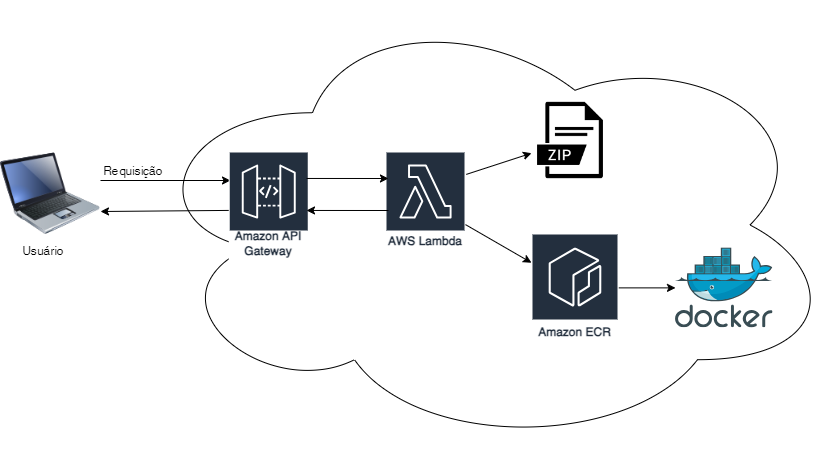
\includegraphics [width=\linewidth]{images/environment-diagram-PT.png}
    \par
    \caption{Diagrama do ambiente de testes}
    \label{fig:env_diagram}
\end{figure}

Por fim, foi montado um \textit{script} na linguagem Python para realizar chamadas às funções via API Rest com um intervo de uma hora dentro no período de um dia. Este intervalo de tempo garante que a função tenha sido desalocado, e portanto, a primeira chamada irá requerer a inicialização da partida lenta.


\subsection{Custo}
\label{subsec:cost}

Para executar todos os testes na AWS, não houve incidência de cobrança do provedor por ter sido utilizado apenas serviços e configurações no nível \textit{Free Tier}. Esse nível possibilita que clientes utilizem serviços de forma gratuita, desde que atendam as restrições existentes. Portanto, para comparar o custo entre as duas abordagens de implantação, são usados os valores base de precificação do provedor de nuvem AWS.

O custo para implantar e manter a função \textit{serverless} ativa é o mesmo, independente da abordagem escolhida. Outros fatores, como configuração de \textit{hardware} e localização do servidor podem impactar no valor final, mas estão fora do escopo deste trabalho.
Ao fazer o \textit{upload} do projeto compactado, não há nenhuma cobrança para armazenar os arquivos. Porém, para disponibilizar uma imagem de contêiner na AWS ECR, há um custo, que é proporcional ao tamanho da imagem. A precificação na AWS ECR também varia dependendo da região \cite{aws_2023_ecr_pricing}. 

\subsection{Desempenho}
\label{subsec:performance}

Algumas métricas podem estar relacionadas ao desempenho de uma aplicação. Neste trabalho, foi analisado o consumo de memória RAM máximo no ambiente ao executar funções \textit{serverless} que estavam em modo de partida lenta. Essa métrica é coletada no console de saída da AWS Lambda ao fazer uma requisição.

Conforme Figura \ref{graph:functions_max_memory_used}, nota-se que o uso de memória máximo com a abordagem de imagem de contêiner se mantém constante, enquanto via arquivo ZIP, há uma variação de uma execução para outra. A Figura \ref{graph:functions_max_memory_used_average} apresenta a média de ambas abordagens, corroborando os resultados da Figura \ref{graph:functions_max_memory_used}, demonstrando que a implantação da função feita a partir da imagem de contêiner obteve melhores resultados em relação ao consumo de memória, ou seja, consome menos memória para executar a função. 

\begin{figure}[H]
    \centering 
    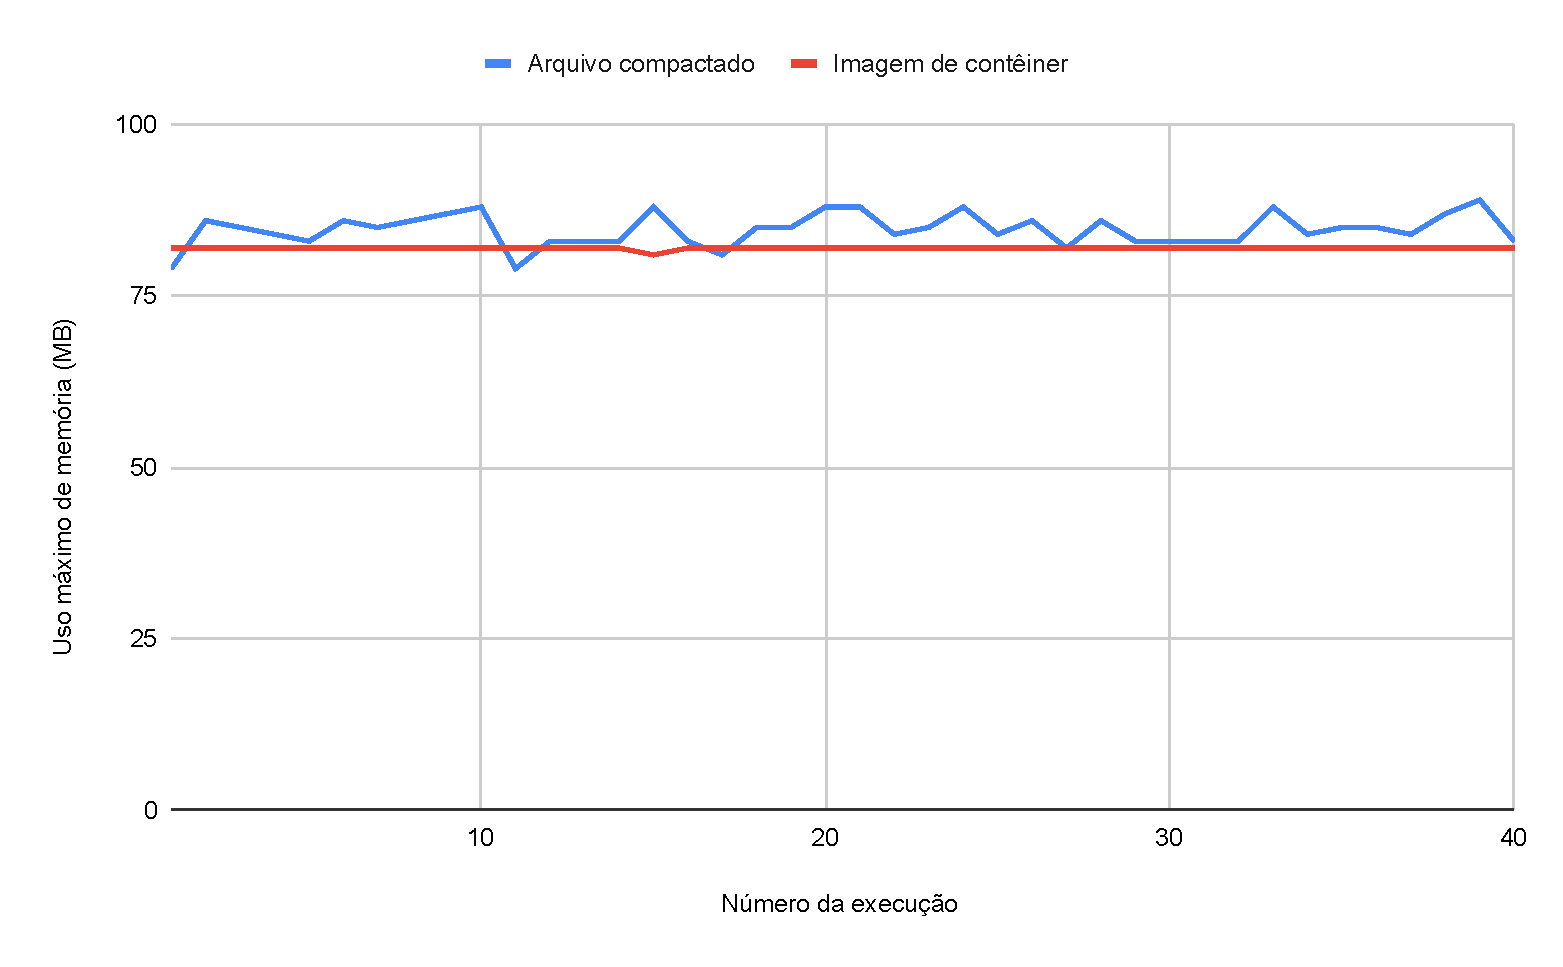
\includegraphics [width=\linewidth]{images/max-memory-use-PT.pdf}
    \par
    \caption{Gráfico de uso de memória máximo em funções \textit{serverless}}
    \label{graph:functions_max_memory_used}
\end{figure}

\begin{figure}[H]
    \centering 
    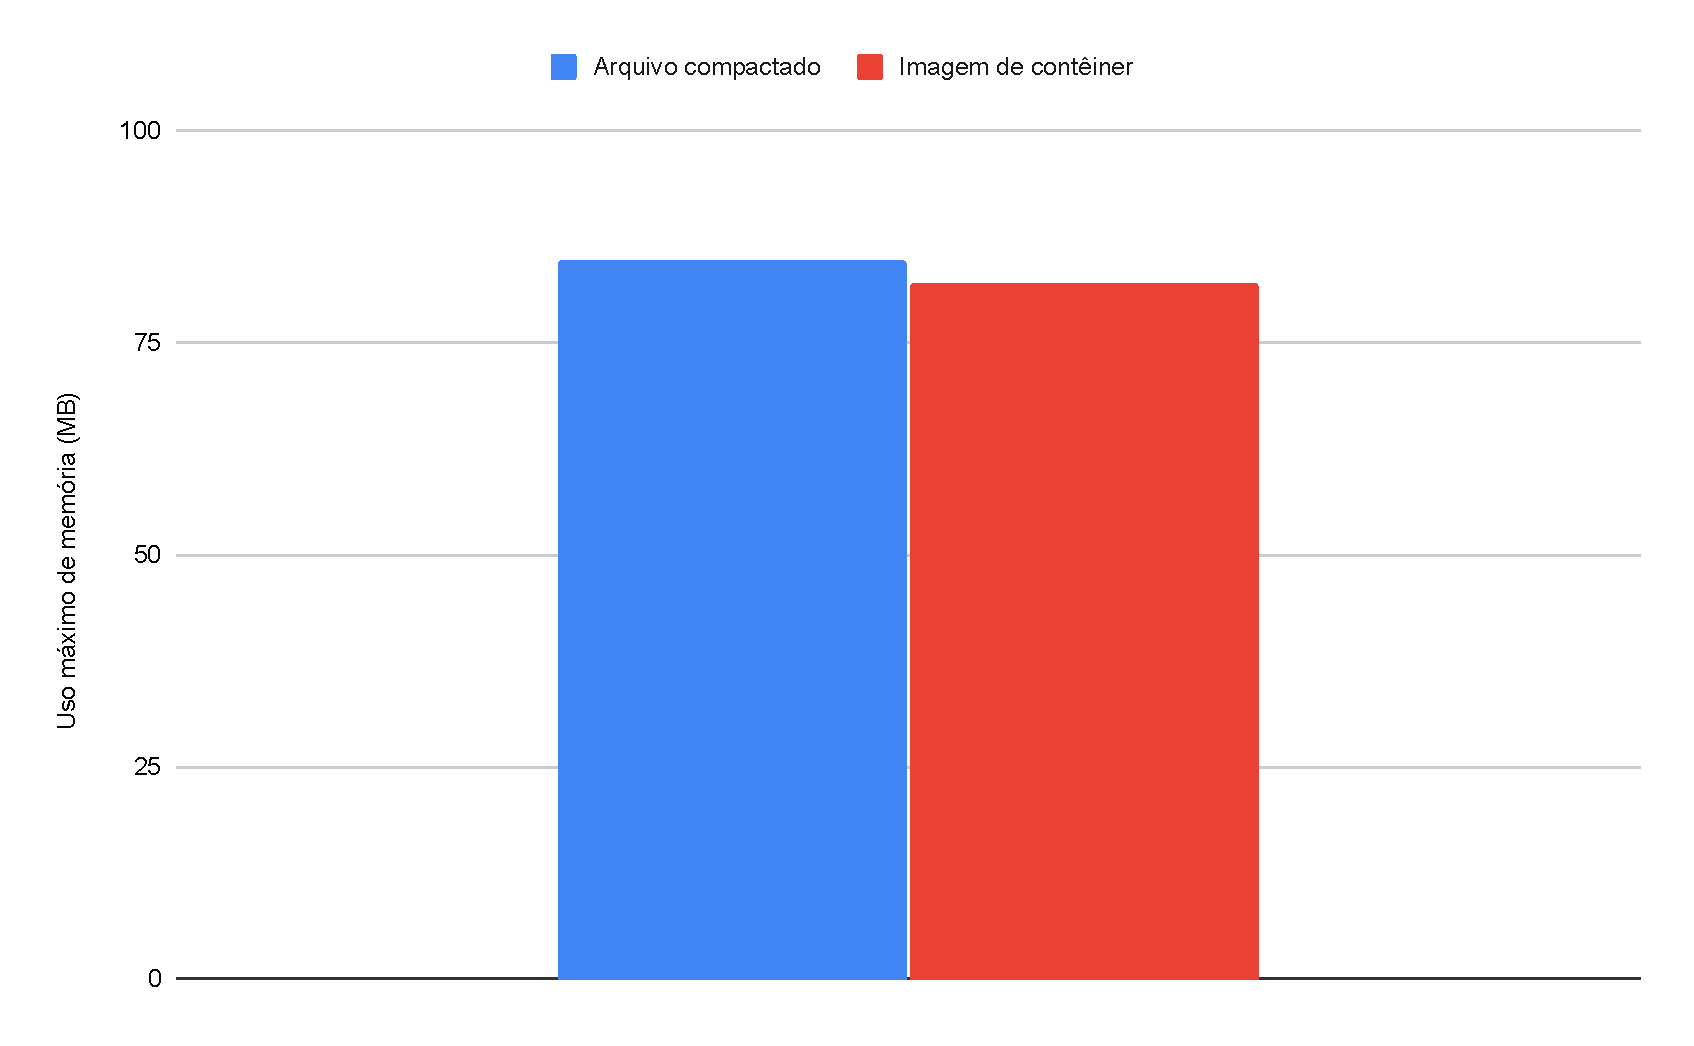
\includegraphics [width=\linewidth]{images/max-memory-use-average-PT.pdf}
    \par
    \caption{Gráfico da média de uso de memória máximo em funções \textit{serverless}}
    \label{graph:functions_max_memory_used_average}
\end{figure}

\subsection{Tempo de inicialização da partida fria} 
\label{subsec:cold_start_time}

As Figuras \ref{graph:functions_init_time} e \ref{graph:functions_init_time_average} mostram que o método de implantação via arquivo ZIP possui o menor tempo de inicialização. Particularmente, observa-se na Figura \ref{graph:functions_init_time} o tempo de inicialização da função implantada via arquivo compactado e via contêiner, para várias inicializações. Cada inicialização ocorreu respeitando tempo suficiente para que os recursos fosses desalocados, obrigando uma nova instanciação da função. A Figura \ref{graph:functions_init_time_average} apresenta a média dos tempos de inicialização apresentados na Figura \ref{graph:functions_init_time}.

O tempo de inicialização também impacta no tempo de resposta quando a aplicação está em modo de partida lenta, portanto, funções executando com arquivo compactado obtém melhores resultados.

\begin{figure}[H]
    \centering 
    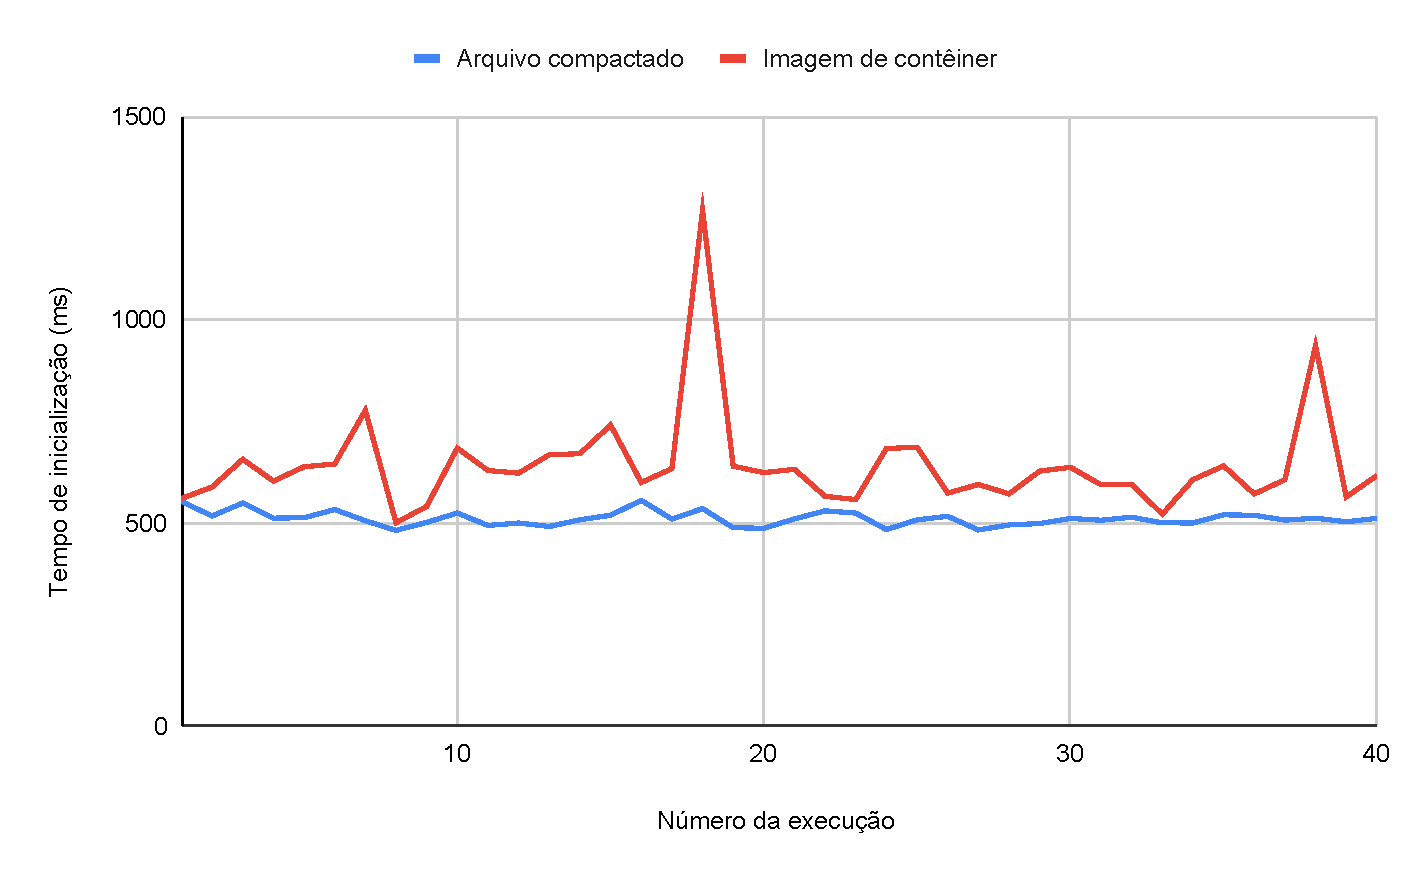
\includegraphics [width=\linewidth]{images/init-time-PT.pdf}
    \par
    \caption{Gráfico do tempo de inicialização em funções \textit{serverless}}
    \label{graph:functions_init_time}
\end{figure}

\begin{figure}[H]
    \centering 
    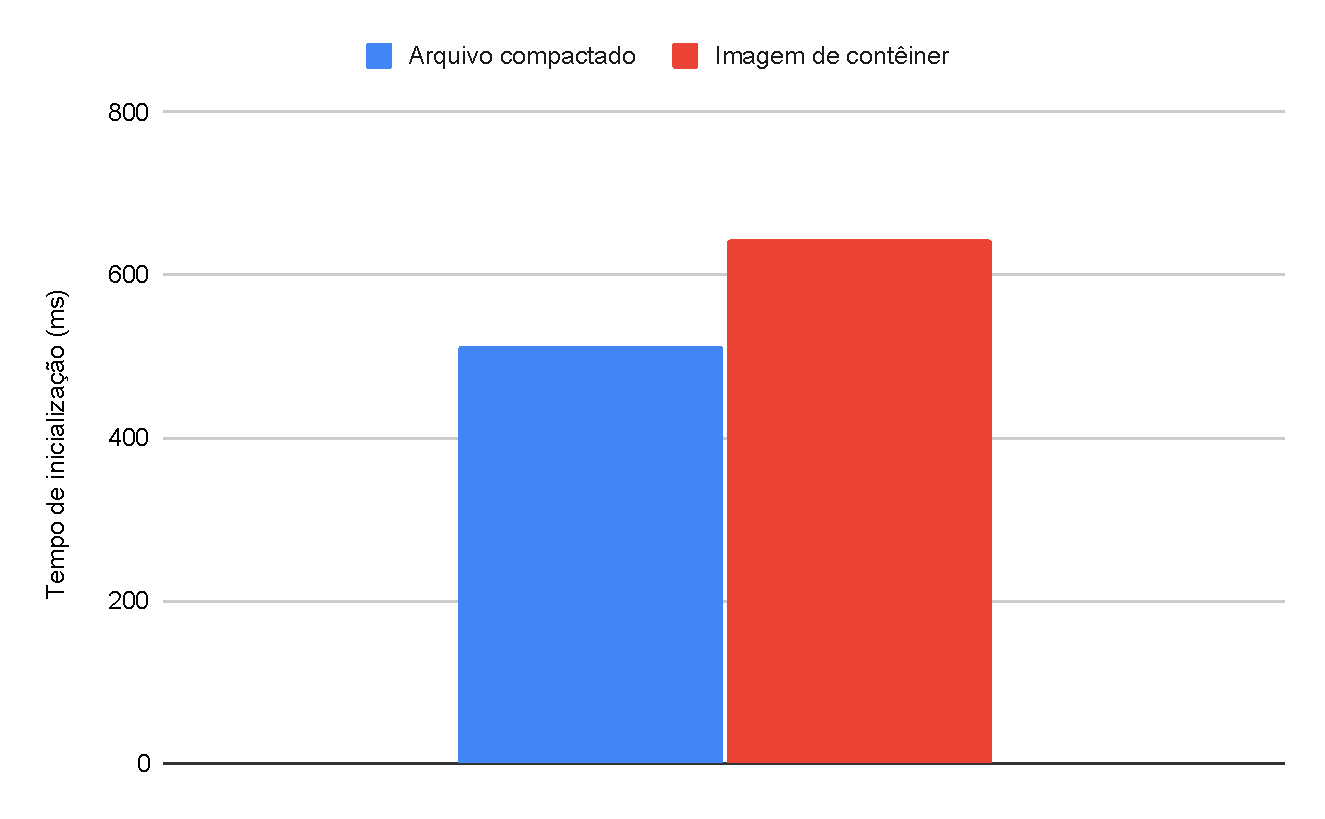
\includegraphics [width=\linewidth]{images/init-time-average-PT.pdf}
    \par
    \caption{Gráfico da média do tempo de inicialização em funções \textit{serverless}}
    \label{graph:functions_init_time_average}
\end{figure}

\section{Conclusão}
\label{sec:Conclusion}

Esse trabalho avaliou os modelos de implantação de funções \textit{serverless} disponíveis na AWS Lambda. O serviço oferece duas possibilidades: via arquivo compactado no formato ZIP e via imagem de contêiner. Com os arquivos compactados ZIP, o modelo de implantação é mais fácil, pois é necessário apenas fazer-se o \textit{upload} do projeto para o serviço AWS Lambda, enquanto na outra abordagem é necessário configurar um arquivo Dockerfile para executar a aplicação, gerar uma imagem de contêiner e publicá-la na AWS ECR.

Dependendo do modelo escolhido, o custo, o desempenho e o tempo de inicialização da partida lenta podem ser diferentes.
Ao criar as funções \textit{serverless} na AWS Lambda nos dois modelos de implantação, ambos não tiverem incidências de custos durante os testes realizados. Porém, quando a abordagem escolhida é com o uso de uma imagem de contêiner, é necessário utilizar outro serviço para armazenar a imagem, nesse caso o AWS ECR, e este pode vir a gerar custos conforme o tamanho da imagem. Ao analisar o uso máximo de memória RAM quando a aplicação está em modo de partida lenta, ambos apresentaram consumo similar, com a vantagem que via imagem de contêiner o uso da memória se manteve constante. A maior diferença se deu no tempo de inicialização da aplicação em partida lenta, no qual a implantação via arquivo ZIP mostrou ser mais eficiente para alocar os recursos e tornar a função ativa novamente.

Portanto, com base nos dados e resultados obtidos e em sua análise, pode-se concluir que a implantação via arquivo ZIP apresenta vantagens. As principais vantagens comparadas ao modelo de implantação com imagem de contêiner são o custo para implantação, uma vez que não é necessário pagamento para armazenar os arquivos compactados e o tempo de inicialização quando em partida lenta é menor.  

Como trabalho futuros, pode-se estender a comparação para as outras linguagens de programação suportadas pelo provedor de nuvem AWS. Outro aspecto a ser comparado é a arquitetura na qual a função \textit{serverless} é executada, x86\_64 ou arm64. Neste trabalho, foi utilizado apenas a arquitetura arm64, havendo espaço para tratar da arquitetura x86\_64. O escopo da aplicação também pode extrapolado para aplicações maiores ou mais complexas que demandem maior processamento computacional, e que deve impactar no consumo máximo de memória e tempo de inicialização.


\bibliographystyle{IEEEtran}
\bibliography{IEEEexample}

\end{document}
